\documentclass[table,xcdraw]{article}
\usepackage[utf8]{inputenc}
\usepackage{tikz}
\usepackage{circuitikz}
\usepackage{float}
\usetikzlibrary{calc}
\usetikzlibrary{positioning,shapes.gates.logic.US}
%\usepackage[table,xcdraw]{xcolor}

\title{Digital Logic Design Assignment 10 - EC2016-17}
\author{Priyansh Agrahari}

\begin{document}

\maketitle

\section{Question}
Assume that all the digital gates in the circuit shown in the figure are ideal, the resistor \textit{R} = 10 \textit{k}$\Omega$ and the supply voltage is 5 \textit{V}. The D flip-flops D$_1$, D$_2$, D$_3$, D$_4$ and D$_5$ are initialized with logic values 0, 1, 0, 1 and 0, respectively. The clock has a 30\% duty cycle.

\begin{figure}[h]
    \centering
    \scalebox{0.65}{
    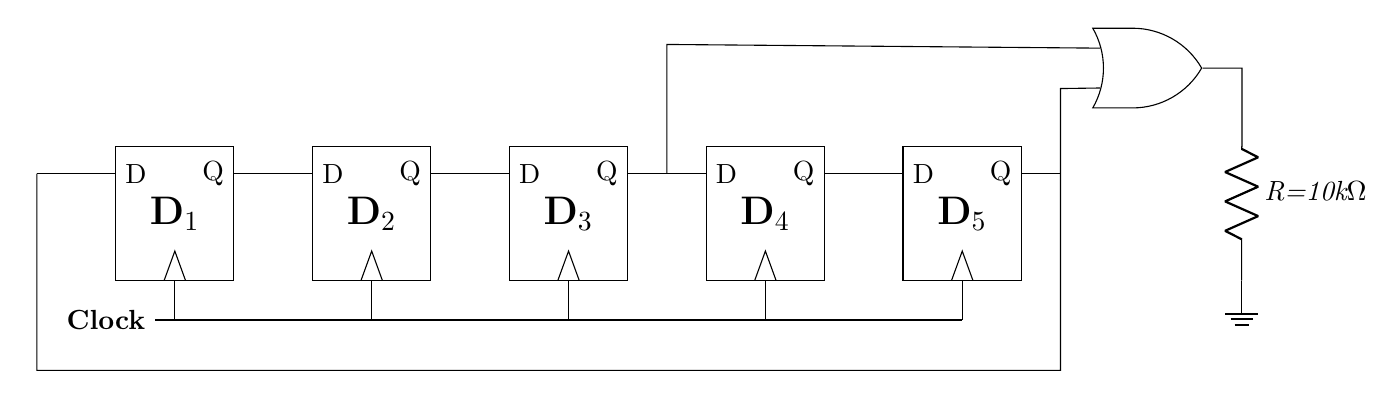
\begin{tikzpicture}[
        GateCfg/.style={
            logic gate inputs={normal,normal,normal},
            draw,
            scale=1.5
        }
    ]
    
    %D flip-flop 1
    \draw (0,0)coordinate (A)--++(0:1.5)coordinate (B)--++(90:1.7)coordinate (C)--++(180:1.5)coordinate (D)--cycle;
    \draw ($(A)!0.5!(C)$)node[]{\Large\textbf{D$_1$}};
    \draw ($(A)!0.8!(D)$)node[right]{D}--++(180:1)node[]{};
    \draw ($(A)!0.5!(B)$)node[above]{}--++(-90:0.5)node[]{};
    \draw ($(A)!0.41!(B)$)node[above]{}--++(70:0.4)node[]{}--++(-70:0.4)node[]{};
    \draw ($(B)!0.8!(C)$)node[left]{Q}--++(0:0.5)node[]{};
    
    %D flip-flop 2
    \draw (2.5,0)coordinate (A)--++(0:1.5)coordinate (B)--++(90:1.7)coordinate (C)--++(180:1.5)coordinate (D)--cycle;
    \draw ($(A)!0.5!(C)$)node[]{\Large\textbf{D$_2$}};
    \draw ($(A)!0.8!(D)$)node[right]{D}--++(180:0.5)node[]{};
    \draw ($(A)!0.5!(B)$)node[above]{}--++(-90:0.5)node[]{};
    \draw ($(A)!0.41!(B)$)node[above]{}--++(70:0.4)node[]{}--++(-70:0.4)node[]{};
    \draw ($(B)!0.8!(C)$)node[left]{Q}--++(0:0.5)node[]{};
    
    %D flip-flop 3
    \draw (5,0)coordinate (A)--++(0:1.5)coordinate (B)--++(90:1.7)coordinate (C)--++(180:1.5)coordinate (D)--cycle;
    \draw ($(A)!0.5!(C)$)node[]{\Large\textbf{D$_3$}};
    \draw ($(A)!0.8!(D)$)node[right]{D}--++(180:0.5)node[]{};
    \draw ($(A)!0.5!(B)$)node[above]{}--++(-90:0.5)node[]{};
    \draw ($(A)!0.41!(B)$)node[above]{}--++(70:0.4)node[]{}--++(-70:0.4)node[]{};
    \draw ($(B)!0.8!(C)$)node[left]{Q}--++(0:0.5)node[]{};
    
    %D flip-flop 4
    \draw (7.5,0)coordinate (A)--++(0:1.5)coordinate (B)--++(90:1.7)coordinate (C)--++(180:1.5)coordinate (D)--cycle;
    \draw ($(A)!0.5!(C)$)node[]{\Large\textbf{D$_4$}};
    \draw ($(A)!0.8!(D)$)node[right]{D}--++(180:0.5)node[]{};
    \draw ($(A)!0.5!(B)$)node[above]{}--++(-90:0.5)node[]{};
    \draw ($(A)!0.41!(B)$)node[above]{}--++(70:0.4)node[]{}--++(-70:0.4)node[]{};
    \draw ($(B)!0.8!(C)$)node[left]{Q}--++(0:0.5)node[]{};
    
    %D flip-flop 5
    \draw (10,0)coordinate (A)--++(0:1.5)coordinate (B)--++(90:1.7)coordinate (C)--++(180:1.5)coordinate (D)--cycle;
    \draw ($(A)!0.5!(C)$)node[]{\Large\textbf{D$_5$}};
    \draw ($(A)!0.8!(D)$)node[right]{D}--++(180:0.5)node[]{};
    \draw ($(A)!0.5!(B)$)node[above]{}--++(-90:0.5)node[]{};
    \draw ($(A)!0.41!(B)$)node[above]{}--++(70:0.4)node[]{}--++(-70:0.4)node[]{};
    \draw ($(B)!0.8!(C)$)node[left]{Q}--++(0:0.5)node[]{};
    
    %OR gate
    \draw (13,2.7)node[or gate US,GateCfg](OR){};
    
    %connections
    \draw (7,1.36)node[]{}--(7,3)node[]{}--(OR.input 1)node[]{};
    \draw (0.5,-0.5)node[left]{\textbf{Clock}}--++(0:10.25)node[]{};
    \draw (-1,1.36)node[]{}--++(-90:2.5)node[]{}--++(0:13)node[]{}--++(90:3.58)node[]{}--(OR.input 3)node[]{};
    \draw (OR.output)node[]{}--++(0:0.5)node[]{}--++(-90:1)node[]{}--(14.3,1.7)to[R,l=\textit{R=10k$\Omega$}] (14.3,0.5)--(14.3,0)node[ground]{};
    
\end{tikzpicture} }
    \caption{\textit{Question figure}}
    \label{fig:ques}
\end{figure}

The average power dissipated (in mW) in the resistor \textit{R} is $\_\_\_\_\_\_\_\_\_\_$
\vfill

\section{Solution}
Let the output waveform be represented by $Y$. Then, we can infer from the question figure that
\begin{equation}
    Y=Q_3+Q_5
\end{equation}

\subsection{Truth Table}
\begin{table}[H]
    \centering
    \renewcommand{\arraystretch}{1.1}
\begin{tabular}{|c|c|c|c|c|c|c|c|}
\hline
\textbf{Clk}             & \textbf{Q$_1$} & \textbf{Q$_2$} & \textbf{Q$_3$} & \textbf{Q$_4$} & \textbf{Q$_5$} & \textbf{Y = Q$_3$ + Q$_5$} \\ \hline
{\color[HTML]{6200C9} 0} & 0              & 1              & 0              & 1              & 0              & 0                          \\ 
{\color[HTML]{6200C9} 1} & 0              & 0              & 1              & 0              & 1              & 1                          \\ 
{\color[HTML]{6200C9} 2} & 1              & 0              & 0              & 1              & 0              & 0                          \\ 
{\color[HTML]{6200C9} 3} & 0              & 1              & 0              & 0              & 1              & 1                          \\ 
{\color[HTML]{6200C9} 4} & 1              & 0              & 1              & 0              & 0              & 1                          \\ 
{\color[HTML]{6200C9} 5} & 0              & 1              & 0              & 1              & 0              & 0                          \\ \hline
\end{tabular}
    \caption{\textit{Truth Table for the Circuit Diagram given in the Question Figure}}
    \label{tab:table}
\end{table}
Now, using the truth table, we can make the timing diagram as given below.

\subsection{Timing Diagram}
\begin{figure}[h]
    \centering
    \resizebox{\columnwidth}{!} {
    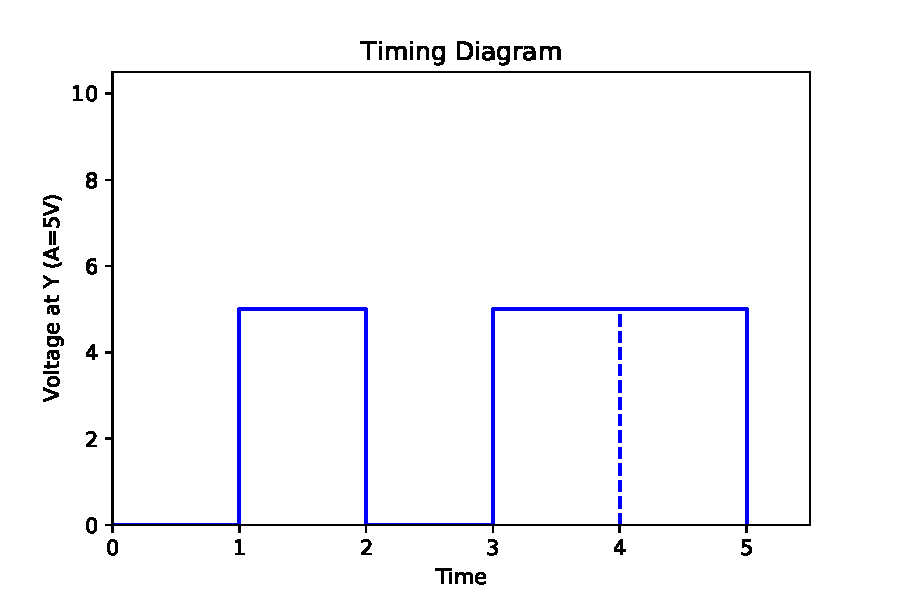
\includegraphics{figs/graph.pdf} }
    \caption{\textit{Timing Diagram for the Circuit Diagram given in the Question Figure}}
    \label{fig:graph}
\end{figure}

Here, the time 0 to 5 represents one time period T of the clock. 
From the timing diagram, we can see that out of the total time, the time for which the voltage across the resistor is non-zero for three division out of five.\par
We can thus calculate the average power using:

\begin{equation}
    Average\:power\:dissipated = P_{avg}=\frac{1}{T}\int_{0}^{T} VI \,dt
\end{equation}
writing $I$ in terms of $V$ (5$V$) and $R$ (10$k\Omega$), we get:
\begin{equation}
    P_{avg}=\frac{1}{T}\frac{V^2}{R}\int_{0}^{T}\,dt
\end{equation}
placing the value of integral, we get:
\begin{equation}
    P_{avg}=\frac{1}{T}\frac{V^2}{R}\frac{3T}{5}
\end{equation}
finally, placing the values of $V$ and $R$, we get:
\begin{equation}
    P_{avg}=\frac{3}{5}\frac{5^2}{10000}
\end{equation}
\begin{equation}
    P_{avg}=1.5
\end{equation}
\vfill
\hrule

\end{document}
